\section{Implementation of Deadbands}
FERC requirements for droop and deadband are 5\% and 36 mHz respectively\cite{ferc2018}.
However, practical implementation is left to generator operators.

\subsection{Types of Deadbands}
Fig. \ref{fig: deadbandType} presents implementations of deadbands that follow FERC requirements.
If a governor has no deadband, a change in output power is requested for any frequency deviation.
A step deadband ignores any frequency smaller than the setpoint $\pm db_1$ and then steps to meet the set droop curve.
A no-step deadband pushes the original droop curve away from the nominal frequency allowing for the droop curve to cross zero at $\pm db_2$ but never return to the step or no deadband droop curve.
To avoid this alternate droop curve, a non-linear deadband is introduced that linearly increases from $\pm \alpha$ to $\pm \beta$, after which it follows the original droop curve.

\begin{figure}[!ht]
	\centering
	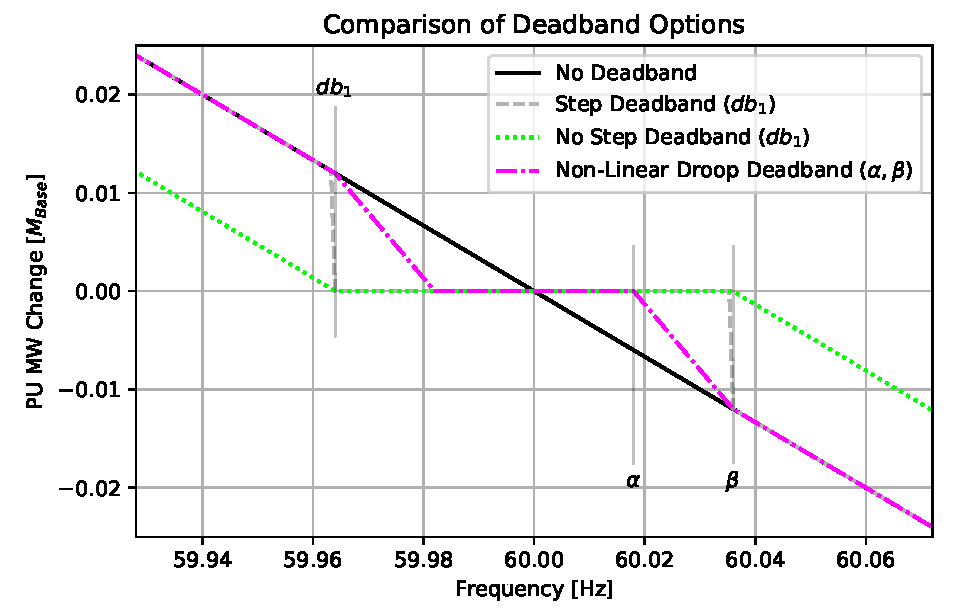
\includegraphics[width=\linewidth]{figures/dbAction3}
	\caption{Different types of deadbands.}
	\label{fig: deadbandType}
\end{figure}